\chapter{Project Background}
\label{chap:antecedentes}


This chapter resumes the main subjects acquired during the accomplishment of the GEO-Cloud project.  The novel architecture proposed in this project for EO processing carries the absence of this kind of platforms to compare with. In this way, the study of the state of the art will be done focalising in some aspects of cloud computing platforms, federated testbeds, networking, satellite systems, and so on. As consequence, this section depicts the different thematic areas .
The conceptual map showed in Figure~\ref{fig:intr-conceptual-map} presents the sections and subsections of this chapter. Thereby in Earth Observation Satellites area, the different concepts for creating and modelling a satellite for earth imaging, its data management and orbital definitions is studied. In high-level languages, some scripting languages are compared. In Networking section, different network impairments and several tools for acquiring these are depicted. In Federated Infrastructre section, the testbeds that Fed4FIRE platform is composed by are explained.

\begin{figure}[!h]
\begin{center}
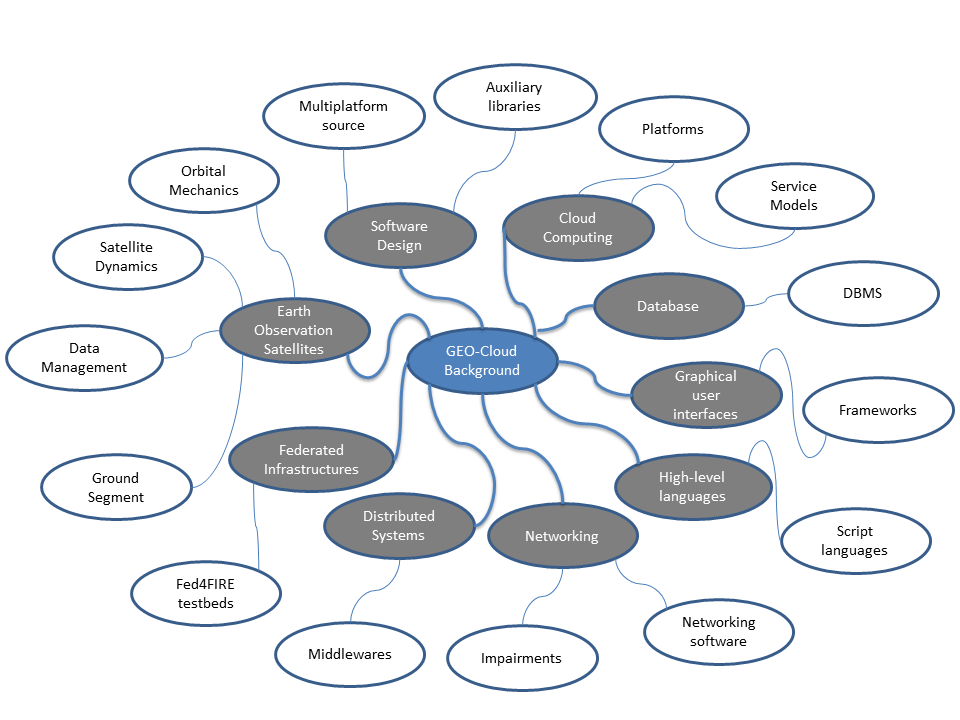
\includegraphics[width=1\textwidth]{statement/background-geocloud.png}
\caption{Conceptual Map of this chapter.}
\label{fig:intr-conceptual-map}
\end{center}
\end{figure}

In the section explains the Graphical User Interfaces background, several
frameworks for developing GUIs are depicted. In Database section, differents
database management systems are compared. The distributed systems section
explains and compares some middlewares as Hadoop or ZeroC Ice for developing
distributed applications.
Finally, in the Software Design section discusses the requirements for building multiplatform code, and other ancillary libraries required by the detailed objectives of GEO-Cloud.

\section{Earth Observation Satellites}

In this section, different areas of aeronautics are involved. Orbital
Mechanics which defines and calculates the satellite orbits for rounding around
the world;  Spatial Telescopes which contributes with the payload parameters as
GSD, Swath among others; finally, the data management which mission consist of processing on fly, storing
and sending the science and ancillary data from satellite to Ground Segment.

\subsection{Orbital Mechanics}

This science~\cite{http://en.wikipedia.org/wiki/Orbital_mechanics} studies the motion of the satellite considered as a point with no
mass in space which is affected by \emph{Newton's Laws of Motion}and \emph{Newton's Law of
Universal Gravitation}.
\emph{The Newton's Law of Universal Gravitation} says that \emph{any two bodies in the
universe attract each other with a force that is directly proportional to the
product of their masses and inversely proportional to the square of the distance
between them.}
%~\cite{http://en.wikipedia.org/wiki/Newton\%27s_law_of_universal_gravitation}

\begin{equation}
F = G* {\frac {m_1*m_2}{r^2}}
\end{equation}
where $F$ is the force between the masses, $G$ is the gravitational constant
($6.67x10^{-11}$), $m_1$ and $m_2$ are the first and second mass respectively
and $r$ is the distance between the centers of the masses.

Orbital Mechanics focuses on the trajectories of the
spacecrafts, maneuvers for orbital acquisition, orbit maintenance, end of life
disposal, etcetera.

Spacecrafts motion  is governed by the \emph{Kepler's Laws of Planetary Motion}
%~\cite{http://en.wikipedia.org/wiki/Kepler\%27s_laws_of_planetary_motion}
which can be derived from \emph{Newton's Laws}. These laws are the following:
\begin{enumerate}
\item The orbit of a planet is an ellipse with the Sun at one of the two foci.
\item A line segment joining a planet and the Sun sweeps out equal areas during
  equal intervals of time.
\item The square of the orbital period of a planet is proportional to the cube
  of the semi-major axis of its orbit.
\end{enumerate}


\subsection{Spatial Telescopes }

The \ac{EO} satellites carry on board telescopes pointing to the Earth in order
to acquire images of the surface. The information can be obtained in several
kinds of spectral bands as visible, near infra-red, thermal, etcetera. This
mission employes visible multispectral telescopes distributed in a constellation of satellites
to obtain daily a global map. For selecting the telescopes, the Swath and \ac{GSD}
have been analised. The number of satellites is dependent on the width of the
swath and the telescope resolution is required to achive quality
images for the mission.

Depending on the spectral bands employed for imaging, the applications are
different. Scientific applications as soil categorization, vegetation analisys,
oceanography use hyperspectral imagers which offers information about hundreds
of bands. 

Other applications as traffic monitoring, urban development,
surveillance commonly require multispectral imagers with visible bands.

\subsection{Data Management}

4 parameters
multiplexing
pre-processing on board for downloading
ancillary data
store and forward sytem for downloading










\section{High-level languages}

For the development of the project, \ac{XML}, Python and Bash languages has
been used. The first, XML, has been used for building the configuration file of
the Orchestrator component and to obtain the selected nodes by JFed
application. The rest of them are scripting languages. The source of the
components of the cloud has been developed using Python and the interconnections
between modules and others secundary funcionalities, in Bash script.

\subsection{XML}
\ac{XML} is a markup language that defines a set of rules for encoding
documents in a format that is both human-readable and machine-readable. Most of
actual software use it for configuring or for updating its configuration on fly.

\subsection{Scripting languages}

The Scripting technics consist of use a interpreted programming language in
order to provide advanced mechanisms for specifying funcionalities of an
application. The most important features of a scripting language are that is not
compiled and it permits effortless development. Also, some interpreted languages
are multiplatform because is not necessary to compile the source for running in
target platform. 


\subsection{Python}
Python is a object oriented language, although permits imperative and functional
programming. It does not need to compile the source because it is
interpreted. It permits a flexible development because it is dynamic type and in
this project, the most important feature why this language has been used,
consist of it is multiplatform. With this feature, the software is able to be
executed in any platform. The current version is 2.7.4 and it offers several
useful and multipourpose libraries as matlib, pthread, mysqllib, pdb and so on.

\subsection{Bash Script}

Really, Bash is not a language, is a command language interpreter for the GNU
operative system. Bash is fully compatible with other command language
interpreters like \emph{sh} or \emph{ksh}, so the source developed by Bash, normally, is
portable. 
However, the Bash language is also known as Bash. The Bash scripts contains
commands for being executed by the interpreter. This way provides a direct line
to communicate with the operative system and to make some funcionalities ad-hoc.
The Bash language consists of several sentences that the operative system is
able to read and translate in order to play a specific action. All the currents
Linux distributions contains a Bash interpret. 


\section{Networking}

For simulating an environment as real as possible in GEO-Cloud, the impairments  of the networks between both Ground Stations and Cloud Platform
and between both Cloud Platform and end-users had to be acquired. Also, features
like bandwidth is obtained in order to stablish the maximum throughput of
channel over \vw.

There are several simulators that
calculates the value of these network feautures roughly but the obtained results
may be wrong o not accurating. Therefore, a subexperiment explained in
Section~\ref{sec:planetlab} for acquiring these values is implemented. 

\subsection{Impairments}

The communication though the Internet is not perfect because there are many
sources or random events that affect traffic packets that are traversing a
network differently at any given moment. This is a main
subject to take into account when a network is being modelling. The main
impairments
%~\cite{http://iwl.com/white-papers/network-impairments/causes-and-correlation}
 of a network are the following:

\begin{itemize}
\item \emph{Packet Loss:} This is simply the disappearance of a packet that was
  transmitted or ought to have been transmitted.
\item \emph{Packet Delay:} Also known as ``Latency'' is the amount of time that elapses between the time a
  packet is transmited to physical environment until the packet is received by
  target. This delay is composed by three types of delay times: Propagation
  delay which is the time that the packet waste arriving destination;
  Routing/Switching delay that is the time that the routers or
  switches waste in processing the packet; finally the Queuing delays that is
  the time that the packet is queued in any intermediate hardware of the entire network.
\item \emph{Jitter:} Jitter is a measure of the variation in the packet delay
  experienced by a numer of packets. 
\item \emph{Packet Duplication:} May occurs when one packet become two or more
  identical packets.
\item \emph{Packet Corruption:} It occurs when the payload of the packet (even a bit)
  is damaged but the packet continues to flow towards the destination instead of
  being discarded.
\end{itemize}

For GEO-Cloud project, the impairments to be acquired are \emph{Packet Loss} and
\emph{Packet Delay} that permit modelling a simulated and close to realily network.


\subsection{Networking Software}

In the networking subject, there are lots of tools that permit to obtain the
features values for the metrics defined above in a network. 
For measuring the throughput, bandwidth and loss-rate the following tools are interesting:

\begin{itemize}
\item \emph{Microsoft's NTttcp~{http://gallery.technet.microsoft.com/NTttcp-Version-528-Now-f8b12769}:} Test tool is effectively iperf on steroids and
  optimized for Windows environments. NTttcp does one better in correlating in
  CPU usage for a network task as well as allowing mapping to CPUs for systems
  with multiple processor capability. 
\item \emph{NetCPS:} Is an oldie but a goodie, and between iperf and NTttcp,
  most basic network testing can be performed to give a good baseline of network
  performance.
\item \emph{Iperf~{https://iperf.fr/}:} the most popular tool to measure maximum TCP bandwidth, allowing the
  tunning of various parameters and UDP characteristics. Iperf reports
  bandwidth, delay, jitter and datagram loss. JPerf is a Java-extension for
  providing a graphical user interface.
\item \emph{Uperf~{http://www.uperf.org/manual.html}:}Is a network
  performance measurement tool that supports execution of workload profiles. It
  is more complex and complete than Iperf or NetPerf allowing the user to model
  a application using a very high level language and running this over the
  network. It allows to use multiple protocols, varying message sizes, to
  collect statistics among others.
\item \emph{NetPerf~{http://www.netperf.org/netperf/}:} Is a benchmark that can be used to measure the performance of many different types of networking. It provides tests for both unidirectional throughput, and end-to-end latency.
\end{itemize}

For measuring the Delay time the following tools are depicted:
\begin{itemize}
\item \emph{Ping:} It is the most used tool for testing the reachability of a host on an
  Internet Protocol network and for measurig the round-trip-time for packets sent
  from a source host to a target host. The sended packets are \ac{ICMP} protocol.
\item \emph{Traceroute:} Is a networking tool for displaying the path and
  measuring transit delays of packets across a network over the Internet
  Protocol. This command is available on a number of moder operative systems. By
  default it works in layer 3 sending \ac{UDP} packets but it can be customized
  for sending \ac{ICMP} packets.
\end{itemize}

\section{Federated Infrastructures}

In this section, some federated infrastructures are depicted. This
infrastructures are used by experimenters for creating new network topologies,
new distributed applications, new network protocols, among others.

A federated infrastructure is a set of unified and autonomous platforms which
are joined in order to provide interoperability and coordinated
information sharing among individual components. 

The federated architecture pattern was first used by the US Federal CIO in
1990s. Then other organizations adopted this paradigm for its infrastructure
technologies. Nowadays, this topology is growing up in business where the
tecnological infrastructure has to be distributed and they must share critical
information around the world.

The benefits of this kind of network topology are enumerated as follows:
\begin{itemize}
\item Independence: the components of the federation has its own rules,
  protocols, subcomponents, and so on. All of them provides a interface for
  communicating among others federation components.
\item For the end-users the federated cloud provides a easily way to host apps
  and the automatically selection of resources from diferent federated components.
\end{itemize}

There are several federated infrastructures for experimenting. These are known
as ``Federated testbeds'' and the most important among others are the following:

\emph{GENI}~{http://ac.els-cdn.com/S1389128613004507/1-s2.0-S1389128613004507-main.pdf?\_tid=320d2494-118e-11e4-9e39-00000aacb35e\&acdnat=1406026495\_7cd6d5a33b3ddfeaf3aad7216039f876}:
The Global Environment for Networking Innovation, is a distributed virtual
laboratory for the future internet sponsored by the U.S. National Science Foundation for
experimentating. In this platform may be carry out developments like protocol
design and evaluation, distributed services, content management and experiments
that needs wide areas\footnote{For more information, see
  \url{http://www.geni.net/}}.

\emph{Open
  Cirrus:}~{http://www.cs.cmu.edu/afs/cs/usr/droh/www/papers/opencirrus-ieeecomputer.pdf}
The Open Cirrus testbed provides a federation in cloud computing for
experimenting. To support these experiments, global services has been added for
providing distributed common services. The experiments that can be carried out
in this testbed are large-scale clustering experiments, machine learning,
scientific computing among others. Open Cirrus is composed by 10 sites in North
America, Europe and Asia and the platform has been developed by the
U.S. National Science Foundation, the University of Illinois, the Karlsruhe
Institute of Technology, the Infocomm Development Authority of Singapore, the
Russian Academy of Sciences, the Electronics and Telecommunications Research
Institute of South Korea, the malaysian Institute of Microelectronic Systems and
Carnegie Mellon University. This project is sponsored by Hewlett-Packard, Intel
and Yahoo!~\footnote{For more information, see \url{http://opencirrus.org}}.

\emph{Fed4FIRE:} The Fed4FIRE is an Integrating Project under the European
Union's \ac{FP7} addressing the work programme topic Future Internet Research
and Experimentation. The project is performed by a consortium of 29 partners
organisations from 8 countries. The Fed4FIRE  proposal consists of to create a
heterogeneous and federated platform with different kinds of services and applications such
cloud computing, grid computing, smart cities, wireless networking and
large-scale experiments. The federation is composed by the following testbeds:


¿COMO PONGO LAS REFERENCIAS HEREEEEE?????
\begin{enumerate}
\item \emph{Virtual Wall:}For creating network topologies. 
\item \emph{PlanetLab Europe:} For experimenting with nodes around the world.
\item \emph{Norbit:} For experimenting with Wi-Fi resources.
\item \emph{w-iLab.t:} This testbed is intended for Wi-Fi and sensor networking experimentation.
\item \emph{NETMODE:} It consists of Wi-Fi nodes connected with some processors
  for networking experimenting.
\item \emph{NITOS:} Is a testbed offered by NITLab and consists of wireless
  nodes bases on open-source software. 
\item \emph{Smart Santander:} This is a large scale smart city deployment in
  Santander city of Spain to experiment Internet of Things. 
\item \emph{FuSeCo:} This testbed provides resources to experiment with 2G,3G
  and 4G technologies.
\item \emph{OFELIA:} For testing and validating research aligned
  with Future Internet Technologies.
\item \emph{KOREN:} It provides programmable virtual network resources with
  necessary bandwith connecting 6 large cities at the speed of 10 Gbps to 20 Gbps. 
\item \emph{BonFIRE:} It is a multicloud tesbed for experimenting.
\item \emph{performLTE:} Is a realistic enviroment for creating experiments
  using the LTE technology.
\item \emph{Community-Lab:} It is a distributed infrastructure for researchers
  to experiment with community networks for creating digital and social environments.
\item \emph{UltraAccess:} It provides several Optical network protocols and
  resources to experiment with QoS features, traffic engineering, virtual LANs
  and so on.
\end{enumerate}

In GEO-Cloud project, the testbeds used for implementing are \vw,\pl and
\bonfire. These facilities are explained in the next sections.

\subsection{Fed4FIRE Testbeds}

In the section above the Fed4FIRE's testbeds has been numerated. Now, the
facilities that are employed in GEO-Cloud are detailed.

\subsection{Virtual Wall}

\vw is an emulation environment for
experimenting with advances networks, distributed software and service
evaluation carryied out by the University of Ghent. It offers the posibility for experimenters to create any type of
network topology, e.g. emulating a large multi-hop topology, client-server
topologies among others and to check algorithms or protocols for subsequent
marketing. 
Two \vw are available: \vw 1 contains 200 servers: 100
quad-cores and 100 eigth-cores; \vw 2 contains 100 dodeca-cores. 

All servers have a management interface and five gigabit ethernet connections
interconnected all of them by switches. On each of these links,the network
impairments as bandwidth, loss-rate and delay can be configured. Also there are some virtual machines for
customising the resources as the experimenter wants. As last, the network
impairments as bandwidth, loss-rate and delay are configurable.  

\subsection{PlanetLab Europe}

PlanetLab Europe is part of the PlanetLab global system, the world's largest
research networking facility, which gives experimenters access to
Internet-connected Linux virtual machines. About 1000 servers conform PlanetLab
platform located in United States, Europe, Asia and elsewhere as Figure~\ref{fig:intr-planetlab-europe} depicts. 
This platform can be used by experimenters in order to develop and to check
distributed systems, network protocols, peer-to-peer systems, network security
and network measurements among others applications.

Through Fed4FIRE, the experimenters are able to reserve and deploy some
PlanetLab Europe resources and to experiment with them.

\begin{figure}[!h]
\begin{center}
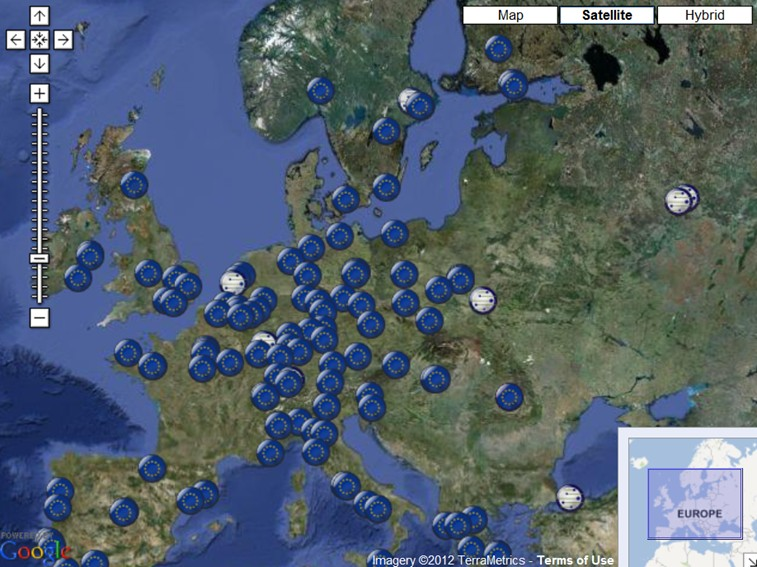
\includegraphics[width=0.6\textwidth]{statement/planetlab-europe.jpg}
\caption{Geographical distribution of PlanetLab Europe.}
\label{fig:intr-planetlab-europe}
\end{center}
\end{figure}

\subsection{BonFIRE}

BonFIRE is a multi-cloud testbed based on an Infrastructure as a Service
delivery model with guidelines, policies and best practices for
experimenting. Currently, BonFIRE is composed by 7 geographically distributed
testbeds, which offer heterogeneous cloud services, compute resources and
storage resources.These testbeds are EPCC, INRIA, Wellness, HLRS, iMinds and
PSNC. The Figure~\ref{fig:intr-bonfire-testbeds} shows these testbeds and its interconnections.

\begin{figure}[!h]
\begin{center}
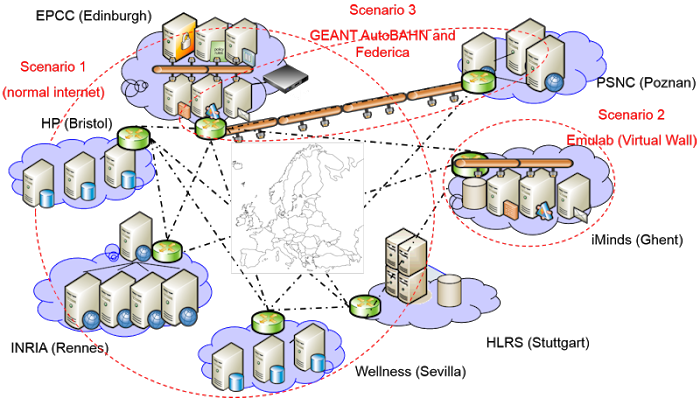
\includegraphics[width=0.7\textwidth]{statement/bonfire-testbeds.png}
\caption{BonFIRE testbeds.}
\label{fig:intr-bonfire-testbeds}
\end{center}
\end{figure}

The compute resources that BonFIRE offers are summarized in Table~\ref{table:intro-instance-types}.

\begin{table}[hp]
  \centering
  {\small
  


\begin{tabular}{p{0.2\textwidth}p{0.2\textwidth}p{0.2\textwidth}p{0.2\textwidth}}
  \tabheadformat
  \tabhead{Name}   &\tabhead{CPU cores} &\tabhead{Memory} & \tabhead{Features}\\
\hline
\textit{Lite}         & 0.5 & 256 MB & \\
\hline
\textit{Small}         & 1 & 1 GB & \\
\hline
\textit{Medium}        & 2 & 2 GB & \\
\hline
\textit{Large}          & 2 & 4 GB & \\
\hline
\textit{Large+}         & 2 & 4 GB & Higher CPU clock speed\\
\hline
\textit{Large-en}        & 4 & 4 GB & \\
\hline
\textit{Xlarge}        & 4 & 8 GB & \\
\hline
\textit{Xlarge+}        & 4 & 8 GB & Higher CPU clock speed\\
\hline
\textit{Custom}        & User defined & User defined &VCPU must be an integer \\
\hline
\end{tabular}


% Local variables:
%   coding: utf-8
%   ispell-local-dictionary: "castellano8"
%   TeX-master: "main.tex"
% End:

  }
  \caption{Instance types of BonFIRE}
  \label{table:intro-instance-types}
\end{table}


   

\subsection{Federated Tools}

The tools for deploying, controlling and monitoring the experiments over
Fed4FIRE are:





\section{Graphical User Interfaces}

\section{Database}

\section{Distributed Systems}

\section{Software Design}




\section{Páginas}
\label{sec:paginas}

La normativa dice que el documento debería ser impreso a una cara, pero si el
número de páginas es alto puede imprimirse a dos caras. Como eso es bastante
subjetivo, mi consejo es que ronde las 100 \textbf{hojas}. Es decir, si el
documento tiene más de 200 páginas imprímelo a doble cara, si tiene menos
imprímelo a una.

Por defecto, \arcopfc{} imprime a una cara (oneside), si quieres imprimir a doble cara,
escribe en el preámbulo:

\begin{listing}
  \documentclass[twoside]{arco-pfc}
\end{listing}

Esto es importante porque a doble cara los márgenes son simétricos y a una cara
no. Si llevas el PFC a la copistería y pides que te lo impriman de modo
diferente al generado, quedará mal ¡Cuidado!
